\chapter{Results and future work}

\section{Experimental results}

To evaluate the proposed method, we conducted experiments using the \textit{SummitXL} robot by \textit{Robotnik}, which is equipped with a laser scanner and IMU sensors. The test environment was a room measuring approximately $7 \times 6$ meters. We moved the robot slowly to minimize noise in the data collected by the IMU.

\begin{figure}[H]
    \centering
    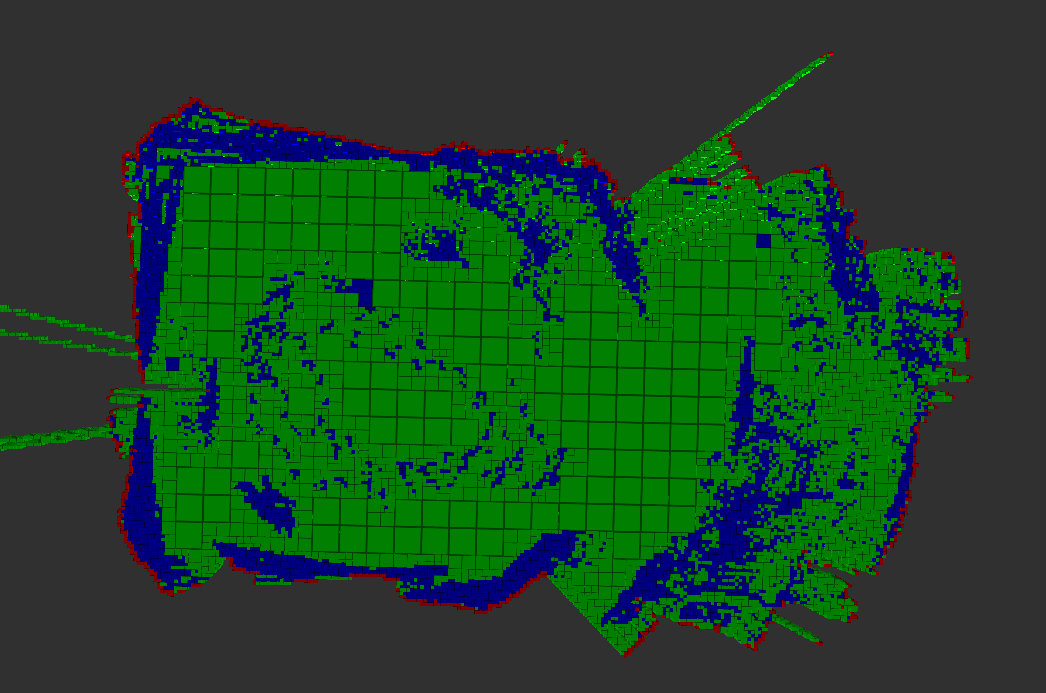
\includegraphics[width=\textwidth]{images/top_screenshot.png}
    \caption{Top view of the octomap generated by our program in the P.E.R.M.I.S. environment. The gray area represents unknown space, the green area represents free space, and the red area represents occupied space. Only the major probability values are shown.}
\end{figure}

In the P.E.R.M.I.S. environment, using the \textit{SummitXL} robot, we obtained the following results:

\begin{itemize}
    \item The octomap provides a coherent representation of the environment, with the boundaries of the room clearly defined.
    \item Moving objects are detected; in the figure, the circle made of blue points represents a person moving around.
    \item Near the room boundaries, the program detects numerous conflicts, likely due to the robot's movement and IMU imperfections.
    \item Attenuation could be useful for detecting moving objects. Occupied cells surrounded by conflict cells often indicate a fixed object, whereas disappearing conflicts usually indicate a moving object.
    \item The program runs in real-time at approximately 15 Hz and could be significantly improved by reducing the resolution.
\end{itemize}

\section{Future work}

The proposed implementation is a first step towards using Evidential Grids for detecting moving objects.
However, several improvements are needed to enhance its efficiency and reliability.

\subsection{Implementation improvements}

Here are the main improvements that could be made to the implementation:

\begin{itemize}
    \item \textbf{GPU acceleration}: The program could be further optimized for faster performance by using GPUs.
    \item \textbf{Standardization of ROS messages}: The lack of standardization in ROS messages is problematic, as different robot manufacturers do not use the laser scan message uniformly.
          This has prevented us from implementing a robust system to filter reliable data.
    \item \textbf{Suitable message for EOGM data}: Despite the existing \texttt{Octomap} message, it is not ideal for further processing of EOGM data.
          One solution could be to use an existing message for RViz and another standardized message for other nodes.
          However, this would sacrifice the size optimization of the \texttt{Octomap} message, leading to slower communication.
          Another solution could be to develop a new message with its own RViz plugin, though this would require significant effort.
\end{itemize}

\subsection{Methodological improvements}

Methodologically, the IMU data exhibits significant noise due to the robot's movements, leading to wide conflict areas, especially near room boundaries.
One potential solution could involve upgrading to a more accurate IMU or implementing methods to mitigate conflicts near fixed objects.
Incorporating SLAM algorithms may enhance robot localization and reduce conflicts.
Additionally, leveraging the robot's movement could aid in detecting moving objects.
For instance, observing the disappearance of conflicts when the robot moves forward could indicate the presence of a moving object.
Furthermore, analyzing the robot's movement patterns could contribute to refining localization accuracy and orientation estimation.